\chapter{Konzept des Prototyps}

In diesem Kapitel wollen wir die Idee hinter unserem Prototypen und die Grundlagen dazu vorstellen. Dabei erklären wir zunächst, um welche Art von Spiel es sich handelt und wie diese umgesetzt werden soll.

\section{Was ist eine Tower Defense?}

In den nachfolgenden Abschnitten wird erläutert, woher Tower Defenses (kurz TDs) kommen, wie das Spielprinzip funktioniert und was die allgemeinen Funktionalitäten einer Tower Defense sind, um einen Überblick über dieses Spiele-Genre zu geben.

\subsection{Spielprinzip und Herkunft}

Die folgenden Angaben sind vergleichbar mit \cite{WIKI01}.

TDs sind ein Subgenre von Echtzeit-Strategiespielen. Dabei soll der Spieler verhindern, dass die Gegner von ihrem Startpunkt zum Zielpunkt gelangen. Dafür werden von dem Spieler Wachtürme oder andere Verteidigungsanlagen gebaut, die automatisch auf die vorbeilaufenden Gegner schießen.

Es gibt zwei grundlegende Arten von TDs:
\begin{description}
\item[Line TD:] \hypertarget{DefinitionLineTD}{Hierbei} laufen die Gegner einen fest definierten Pfad entlang, auf dem der Spieler keine Türme errichten kann. Diese werden stattdessen am Rand des Pfades gebaut, um von dort auf die Gegner zu schießen und sie aufzuhalten.\\
Siehe \autoref{fig:LaneTDSample_KingdomRush} für das Beispiel einer Line TD.
\item[Mazing TD:] \hypertarget{DefinitionMazingTD}{Bei} einer Mazing TD (engl. \textit{maze} "Labyrinth") gibt es einen festen Startpunkt, bei dem die Gegner erscheinen, und einen festen Zielpunkt, den man verteidigen muss. Dazwischen ist eine begrenzte Fläche auf der die Türme errichtet werden können. Mit Hilfe der Verteidigungsanlagen baut der Spieler ein Labyrinth und legt so den Weg der Gegner fest.\\
Dabei müssen Maßnahmen ergriffen werden, um zu verhindern, dass der Spieler den Weg blockiert. Entweder können die Gegner die Türme angreifen, um sich bei Bedarf einen Weg zu öffnen. Oder es wird vor jedem Turmbau geprüft, ob dieser den Weg blockieren würde, sodass dessen Errichtung verboten werden kann.\\
Siehe \autoref{fig:MazeTDSample_DesktopTD} für das Beispiel einer Maze TD.
\end{description}

~\\
Beide Arten stellen den Spieler vor unterschiedliche Herausforderungen. Bei einer Line TD kann man keinen Einfluss auf den Weg der Gegner nehmen, was den Schwierigkeitsgrad eines Levels bestimmt. Zum Beispiel ist ein gewundener Pfad leichter zu verteidigen, als eine gerade Linie, da zum einen die Strecke der Gegner länger ist und der Angriffsbereich eines Turmes effektiver genutzt werden kann.\\
Deswegen muss man sich bei Line TDs genau überlegen, wo man welchen Turm platziert.

Die Möglichkeit bei Maze TDs den Pfad der Gegner selbst festzulegen ist Vor- und Nachteil zugleich. Zum Einen kann so die zurückzulegende Distanz der Gegner maximiert werden und deren Weg an die eigene Strategie angepasst werden, allerdings muss man nun gleichzeitig auf die Konstruktion des Labyrinths und die Art der Türme achten.\\
Das in Kombination damit, dass zunächst eine geeignete Strategie entwickelt werden muss, kann einen schnell überfordern.

Gegner erscheinen in unterschiedlich großen Gruppen, die in zeitlichem Abstand eintreffen. Eine einzelne Gruppe wird auch Wave (engl. \textit{wave} "Welle") genannt. Die Angreifer sind meistens wehrlos, solange man ihnen nicht den Weg versperrt, und laufen einfach ihren Pfad entlang.\\
Erreichen sie ihr Ziel, verliert der Spieler eine, je nach Gegner unterschiedliche, Menge von Lebenspunkten. Sinken diese auf null hat er die Runde verloren.

\newpage
\begin{figure} [t]
\centering
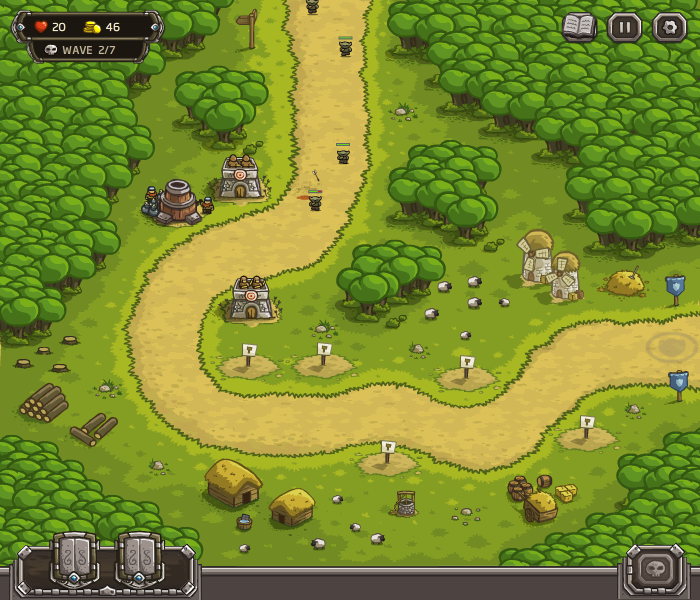
\includegraphics[width=0.67\linewidth]{./images/Kapitel_PrototypKonzept/LaneTDSample_KingdomRush.png}
\caption[Beispiel einer Line TD]{Beispiel einer Line TD anhand von \textit{Kingdom Rush}\\
Die Gegner kommen von oben und laufen den Weg entlang, um zu ihrem Ziel auf der reichten Seite zu kommen. Die Wachtürme am Wegesrand versuchen diese aufzuhalten.}
\label{fig:LaneTDSample_KingdomRush}
\end{figure}
\begin{figure}[b]
\centering
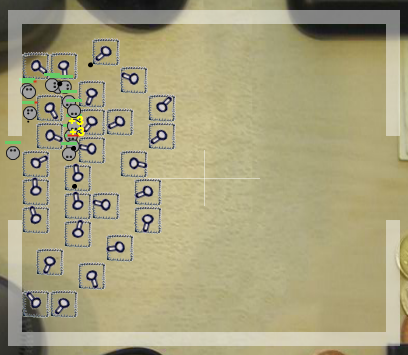
\includegraphics[width=0.67\linewidth]{./images/Kapitel_PrototypKonzept/MazeTDSample_DesktopTD.png}
\caption[Beispiel einer Maze TD]{Beispiel einer MazeTD anhand von \textit{Desktop TD}\\
Die Gegner laufen von links nach rechts. In dem vom weißen Rand begrenzten Gebiet können Türme errichtet werden, um die Strecke der Gegner zu maximieren.}
\label{fig:MazeTDSample_DesktopTD}
\end{figure}
\clearpage

Eine der ersten TDs war ein Teil des Strategiespiels \textit{Dune 2}, bei dem man seine Basis mit Hilfe von Labyrinthen aus Wachtürmen und Mauern gegen die angreifenden Gegner verteidigen musste.\\
Mit dem umfangreichen und komplexen Karten-Editor von Starcraft, war es den Fans möglich das Spielprinzip von \textit{Starcraft} so stark zu verändern, dass völlig neue Spiele entstanden sind. Ein Teil dieser Fan-Karten waren TDs, wodurch diese zunehmend bekannter wurden.\\
Mit dem Erscheinen von \textit{Warcraft III} wurde der Karten-Editor wesentlich benutzerfreundlicher und umfangreicher, wodurch TDs immer bekannter wurden.\\
Inzwischen gibt es sehr viele TDs in Form von Flash-Spielen, wie zum Beispiel \textit{Kingdom Rush}\footnote{Homepage von Kingdom Rush: \url{http://kingdomrush.com/index.php}} oder \textit{GemCraft}\footnote{Homepage von Gemcraft: \url{http://www.gameinabottle.com/gemcraft1.php}}, und auch einige alleinstehende Spiele, wie zum Beispiel \textit{Plants vs. Zombies}.

\subsection{Funktionalitäten}

Mit der Zeit haben sich viele neue Funktionalitäten für TDs entwickelt. Hier werden die grundlegenden erläutert und es wird auch auf einige weiterführende eingegangen.

Eine TD besteht normalerweise aus mehreren Levels, in denen der Pfad der Gegner unterschiedlich ist, um das Spiel abwechslungsreicher zu gestalten und den Schwierigkeitsgrad zu variieren.\\
Mit Beginn jedes Levels beginnt der Turmbau von vorne. In manchen TDs kann man Errungenschaften aus vorherigen Levels während des Spielverlaufs behalten. Dies sind zum Beispiel Erfahrungspunkte, besondere Fähigkeiten oder allgemeine Verbesserungen der Verteidigungsanlagen.\\
Mit steigendem Level treten immer stärkere Gegner auf, allerdings werden auch bessere Verteidigungsanlagen freigeschaltet, oder das Einkommen steigt, um mehr bauen zu können.

\paragraph{Verteidigungsanlagen} In jeder TD gibt es verschiedene Verteidigungsanlagen, welche sich durch ihre Angriffsreichweite, Angriffsgeschwindigkeit, Angriffsart und ihren Schaden unterscheiden.\\
Verschiedene Angriffsarten sind zum Beispiel Angriffe, die einzelnen Gegnern Schaden zufügen (z.B. Bogenschützen) und welche die Flächenschaden um ihren Treffpunkt verursachen (z.B. Katapulte). Des Weiteren kann man durch die Flugbahn und den Schadenstyp differenzieren. Manche Türme schießen zielsuchende Geschosse, während andere versuchen die Position des Gegners zu schätzen, um ihn dadurch zu treffen. Einige verfügen auch über Spezialfähigkeiten, um den Gegner zum Beispiel zu verlangsamen oder zu vergiften.\\
Türme können unterschiedliche \hypertarget{Schadensarten}{Schadensarten} verursachen, die je nach Rüstungsart des Gegners mehr oder weniger Schaden verursachen. Beispielsweise würde \textit{Feuerschaden} bei durch \textit{Natur} geschützte Gegner einen erhöhten Schaden verursachen, während bei Gegnern mit \textit{Wasserrüstung} nur noch ein niedriger Schadenswert zugefügt werden würde. Meistens wird dabei das Schere-Stein-Papier-Prinzip\footnote{Das Schere-Stein-Papier-Prinzip bedeutet, das eine Schadensart zwar einer Rüstungsart überlegen, einer anderen jedoch unterlegen ist [\url{http://de.wikipedia.org/wiki/Schere,\_Stein,\_Papier\#Schere-Stein-Papier-Prinzip}, 24.11.2012].} verwendet, was den taktischen Tiefgang erhöht.\\
Es kann auch \hypertarget{DefinitionVerteidungsanlageTypen}{Verteidigungsanlagen} geben, die auf bestimmte \hyperlink{DefintionGegnertypen}{Gegnertypen} spezialisiert sind. Zum Beispiel gibt es Türme die nur Gegner angreifen können, die sich auf dem Boden befinden oder welche die nur Gegner angreifen können, die sich in der Luft fortbewegen. Diese richten bei dem entsprechenden Gegnertyp einen höheren Schaden an, um ihren Nachteil auszugleichen. 

Zusätzlich zu Türmen gibt es manchmal auch Fallen die - auch bei \hyperlink{DefinitionLineTD}{Line TDs} - auf dem Weg der Gegner gebaut werden und auslösen, sobald ein Feind darüber läuft. Diese können wie die Türme Schaden verursachen, oder die Eigenschaften des Getroffenen verschlechtern.\\
In neueren TDs gibt es zunehmend auch \hypertarget{DefinitionMobileEinheit}{mobile Einheiten}, die der Spieler ausbilden kann, um die Gegner an bestimmten Stellen in Kämpfe zu verwickeln und dadurch die Angriffe der Türme effektiver zu machen.

Um Verteidigungsanlagen errichten zu können benötigt man mindestens eine Ressource. Da diese nicht meistens mehr verschoben werden können, sollte die Position wohl überlegt sein. Sie können zwar wieder abgerissen werden, dabei erhält man meist nur einen Teil des investierten Betrags zurück. Ressourcen verdient der Spieler meistens durch ein festes Einkommen und durch das Aufhalten der Gegner.\\
Verteidigungsanlagen lassen sich aufrüsten, wodurch deren Eigenschaften verbessert werden. Dabei gibt es öfters mehrere Auswahlmöglichkeiten, zum Beispiel eine größere Reichweite oder ein höherer Schaden. Selten haben TDs ein Erfahrungssystem für die Türme, wodurch Verteidigungsanlagen, die viele Feinde töten, automatisch stärker werden.

\paragraph{Gegner} unterscheiden sich wie die Verteidigungsanlagen durch ihre Eigenschaften. Diese sind normalerweise die Lebenspunkte, die Rüstungspunkte, die Bewegungsgeschwindigkeit, spezielle Fähigkeiten und in manchen Fällen auch noch die Rüstungsart. Diese hält je nach Schadensart unterschiedlich viel Schaden ab, wie es bereits bei den \hyperlink{Schadensarten}{Verteidigungsanlagen} beschrieben wurde.\\
Wenn man diese Eigenschaften verändert, kann man spezielle \hypertarget{DefintionGegnertypen}{Gegnertypen} erstellen. Diese können zum Beispiel besonders schnelle Gegner, fliegende Gegner oder \textit{Bossgegner} sein. Fliegende Gegner zeichnen sich dadurch aus, dass sie sich nicht auf dem Boden fortbewegen, was als Spezialfähigkeit gesehen werden kann. Dies hat in den verschiedenen TD-Arten unterschiedliche Auswirkungen. In einer \hyperlink{DefinitionLineTD}{Line TD} können in der Regel \hyperlink{DefinitionVerteidungsanlageTypen}{spezielle Türme} gebaut werden, um fliegende Gegner einfacher aufzuhalten. In \hyperlink{DefinitionMazingTD}{Mazing TDs} sind die Auswirkungen schwerwiegender, da fliegende Gegner nicht an das Labyrinth des Spielers gebunden sind, sondern dieses einfach überfliegen. Hier sind spezialisierte Türme essentiell, um nicht zu verlieren.\\
\textit{Bossgegner} sind vergrößerte Versionen normaler Gegner, die wesentlich mehr Lebenspunkte und einen höheren Rüstungswert haben. Zusätzlich dazu können sie Spezialfähigkeiten haben, zum Beispiel dass sie sich nach ihrem Tod in kleinere Versionen aufspalten.\\
\\
Die genannten Funktionalitäten sind natürlich nur ein Bruchteil des Möglichen und von dem was bereits umgesetzt wurde.
\pagebreak

\section{Konzept}\label{sec:Konzept}

Da der Schwerpunkt dieser Studienarbeit bei der testgetriebenen Entwicklung eines Spiels liegt, haben wir uns bei dem Prototypen auf die eine essentielle Funktionalität einer Tower Defense beschränkt. Nämlich den Gegner mittels einer Verteidigungsanlage davon abzuhalten sein Ziel zu erreichen. Um den Programmieraufwand in Grenzen zu halten, haben wir beschlossen, dass es keine Benutzeroberfläche und Benutzerinteraktion geben wird, sondern dass alle notwendigen Elemente bereits zu Spielbeginn vorhanden sind.\\
Die Hauptaufgabe besteht darin, das Verhalten der benötigten Elemente testgetrieben zu entwickeln.

Auch die Darstellung und das Level-Design soll einfach gehalten werden. Der Gegner soll einen geraden Pfad zu seinem Ziel überqueren, wobei in der Mitte des Pfades ein Turm steht. Dieser soll den Gegner aufhalten. Eine schematische Darstellung dieser Szene befindet sich in der nachfolgenden Abbildung.\\

\begin{figure}[h]
\centering
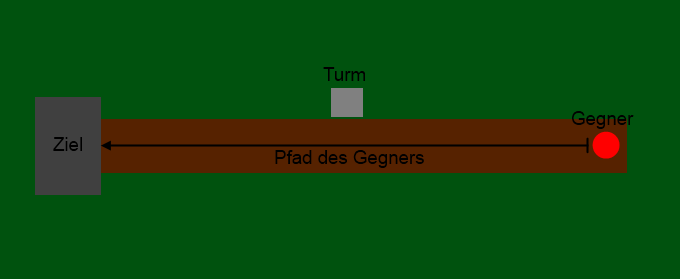
\includegraphics[width=1\linewidth]{./images/Kapitel_PrototypKonzept/Schematischer_Aufbau_der_Szene.png}
\caption[Schematischer Aufbau der Szene]{Schematischer Aufbau der Szene}
\label{fig:Schematischer_Aufbau_der_Szene}
\end{figure}

Es müssen die Funktionalitäten des Prototyps entwickelt werden. Diese sind unter anderem der \textbf{Turm} mit einem \textbf{Angriff} und der \textbf{Gegner} mit einer \textbf{Bewegung}. Um den Code modularer zu gestalten und die Wiederverwendbarkeit zu erhöhen, soll dabei nach dem Prinzip \textit{Favour Composition over Inheritance} (dt.: "Verwende Komposition an Stelle von Vererbung") gearbeitet werden.\\
Für das Konzept ist das nachfolgende Klassendiagramm entstanden, welches einen Überblick über die Struktur des Prototyps schafft und als Orientierung für die Entwicklung dienen soll. Dabei ist zu beachten, dass die Struktur sehr zukunftsorientiert ist, um die später eventuell nötigen Änderungen zu minimieren.\\

\begin{figure}[h]
\centering
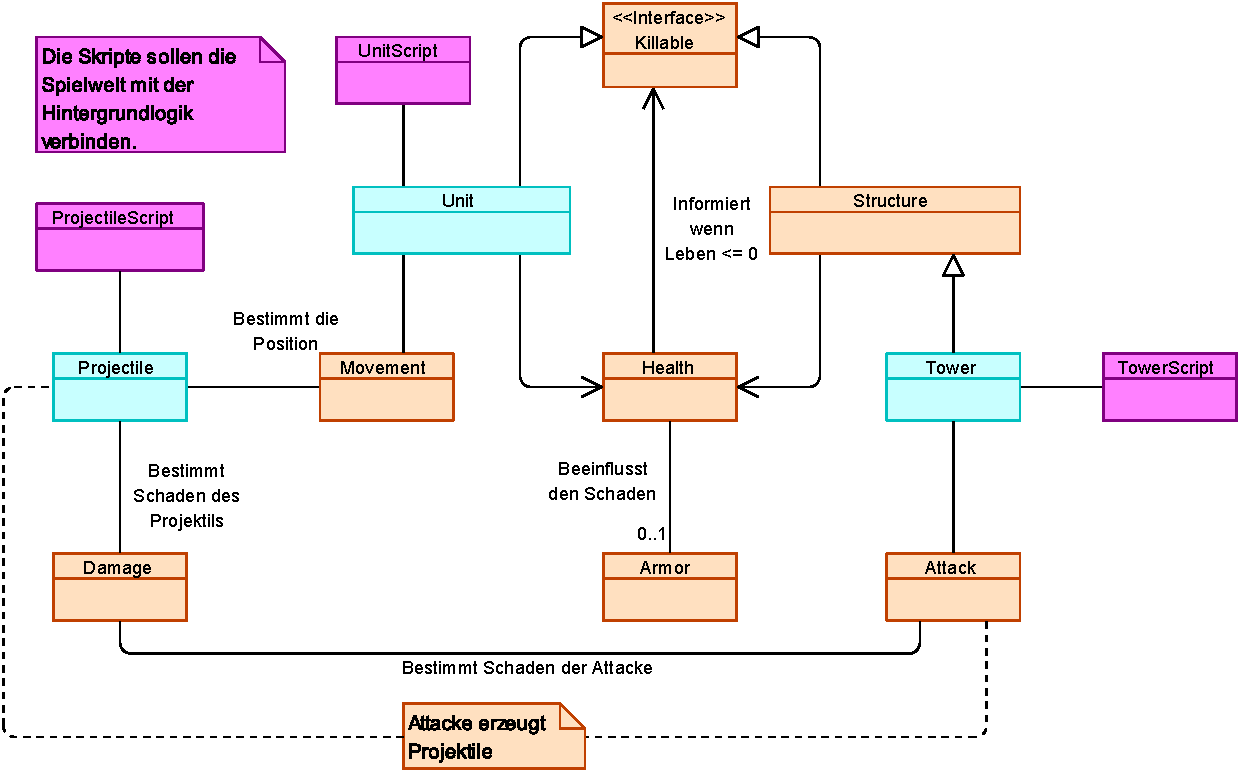
\includegraphics[width=1\linewidth]{./images/Kapitel_PrototypKonzept/Grobstruktur.pdf}
\caption[Grobstruktur des Prototyps]{Grobstruktur des Prototyps\\
Enthält Klassen für die \textbf{\textcolor{ScriptClass}{Skripte}}, die \textbf{\textcolor{ScriptLogicInterface}{Logik-Skript-Schnittstellen}} und die reinen \textbf{\textcolor{LogicClass}{Logik-Klassen}}.
Dieses Diagramm soll als Orientierung für die Entwicklung des Prototyps dienen.}
\label{fig:Grobstruktur}
\end{figure}

Die Klassen des Diagramms lassen sich in drei Bereiche unterteilen.\\
Zum einen die \textbf{\textcolor{ScriptClass}{Skript}}-Klassen, welche an die Spielobjekte angefügt werden und so deren Verhalten direkt beeinflussen (z.B. \textit{TowerScript} oder \textit{UnitScript}).\\
Dazu kommen die Klassen, die den Zustand der Spielobjekte beinhalten und verändern, sowie die nötigen Berechnungen durchführen (z.B: \textit{Health} oder \textit{Movement}). Diese werden in Zukunft als \textbf{\textcolor{LogicClass}{Logik}}-Klassen bezeichnet.\\
Als letztes gibt es noch die Klassen, die den Skripten Zugriff auf die Logik geben und im nachfolgenden \textbf{\textcolor{ScriptLogicInterface}{Logik-Skript-Schnittstellen}} genannt werden (z.B. \textit{Projectile} oder \textit{Unit}). Diese enthalten auch Informationen über den Zustand des Spielobjekts und sind somit auch ein Teil der Logik.

Die Skript-Klassen enthalten immer eine Referenz auf eine Skript-Logik-Schnittstelle, um an den Zustand des Spielobjekts zu gelangen. Dieser wird bei jedem Frame zunächst auf den neusten Stand gebracht, indem die vergangene Zeit an die Schnittstelle übermittelt wird. Dies wird benötigt, um zum Beispiel eine Bewegung auszuführen, da die Position aktualisiert werden muss.\\
Das Skript holt sich den neuen Zustand aus der Schnittstelle und synchronisiert das Spielobjekt damit (Objekt wird auf die aktuelle Position verschoben). Dadurch enthalten Skripte wenig bis keine Logik, sondern müssen nur die Zustände abgleichen. Als Folge ist die Spiellogik unabhängiger von der Game-Engine und lässt sich mit den Standard Unit-Tests für C\# testen.

Die Klasse \textit{Health} repräsentiert die Lebenspunkte eines Objekts. Sie hat eine optionale \textit{Armor}, welche den zugefügten Schaden beeinflusst. Außerdem hat sie eine Referenz auf ihren Besitzer, welcher das \textit{Killable}-Interface implementieren muss, um diesem mitteilen zu können, falls die Lebenspunkte auf null sinken.\\
\textit{Movement} ist dafür zuständig, die Position eines Objekts zu bestimmen. Dabei ist es vorstellbar, dass es unterschiedliche Formen der Bewegung gibt. Zum Beispiel bewegen sich Gegner linear vorwärts, während das Geschoss eines Katapults eine parabolische Flugbahn durchführen würde. Für zielsuchende oder magische Projektile wäre auch eine verfolgende Bewegung denkbar.\\
\textit{Damage} soll Objekten Schaden zufügen und somit mit \textit{Health} wechselwirken.\\
\textit{Projectile} repräsentiert die Geschosse von Türmen und hat eine Bewegung, sowie einen Schaden, den sie dem getroffenen Objekt zufügt. Das \textit{ProjectileScript} soll die Bewegung des Geschosses durchführen und einen Treffer registrieren.\\
\textit{Attack} stellt den Angriff eines Turms dar und erzeugt Projektil-Objekte, wenn auf einen Gegner geschossen wird.\\
\textit{Structure} hat Lebenspunkte und implementiert deswegen das \textit{Killable}-Interface. Diese Klasse ist für unseren Prototypen nicht notwendig, allerdings wäre es vorstellbar, dass der Spieler Blockaden errichten könnte, welche die Gegner zerstören müssen, um ihren Weg fortzusetzen. Oder das Ziel der Gegner ist die Basis des Spielers, welches durch ein \textit{Structure}-Objekt realisiert wird. Erreichen sie die Basis wird ihr Schaden zugefügt und wenn sie zerstört wird, ist das Spiel verloren.\\
\textit{Tower} repräsentiert eine Verteidigungsanlage des Spielers. Sie erbt von \textit{Structure}, wodurch sie Lebenspunkte hat. Dies könnte später dazu verwendet werden, Gegnern die Möglichkeit zu geben, Türme zu attackieren. Des Weiteren hat \textit{Tower} einen (oder später möglicherweise mehrere) Angriff(e), um auf die Gegner zu schießen. Das \textit{TowerScript} soll dem Turm mitteilen, sobald ein Gegner in Reichweite ist oder diese verlässt, sodass dieser angegriffen, beziehungsweise der Angriff gestoppt wird.\\
Die Klasse \textit{Unit} soll einen Gegner darstellen und hat dementsprechend ein \textit{Health}-Objekt und ein \textit{Movement}-Objekt als Attribute. Das \textit{UnitScript} soll die Position des dazugehörigen Spielobjekts aktualisieren, damit es sich auch in der Spielwelt bewegt. Später wäre es sinnvoll, Gegner durch eine Unterklasse von \textit{Unit} (z.B. \textit{Creep}) zu repräsentieren, da es auch neutrale oder befreundete Einheiten geben könnte. Oder der Spieler bekommt die Möglichkeit \hyperlink{DefinitionMobileEinheit}{mobile Verteidigungsanlagen} zu errichten.

Diese Struktur möchten wir im nachfolgenden testgetrieben entwickeln, um einen laufenden Prototypen nach dem Schema in \autoref{fig:Schematischer_Aufbau_der_Szene} zu erhalten.
